There are multiple ways to approach discretizing the ellipse, the most apparent of which being
\begin{equation}\label{eq:parametric_ellipse}
  \xtt = a\cos{\eta} + ib\sin{\eta}, \qquad \eta \in [0, 2\pi),
\end{equation}
where the parameter $\eta$ is the very same as the elliptic coordinate, called the \emph{eccentric} variable.
It is indeed related to the polar variable, as is clear upon considering $\tan{\eta}$.
This value is equal to $\sfrac{az}{bx}$, by the geometric interpretation of the tangent, where $\xtt = x + iz$.
For a polar representation
\begin{equation}\label{eq:polar_ellipse}
\xtt = r\cos{\theta} + ir\sin{\theta}, \qquad \theta \in [0, 2\pi),
\end{equation}
we find that
\[
\tan{\eta} = \sfrac{a}{b} \tan{\theta}, \quad r(\theta) = \frac{ab}{\sqrt{b^2 \cos^2{\theta} + a^2 \sin^2{\theta}}}.
\]
For the circle, when $a = b$, the eccentric and polar angles are of course equal.
We plot the relationship between the eccentric and polar variables, illustrated in figure \ref{fig:eccentric_versus_polar}.
\begin{Figure}
  \centering
  \scalebox{1}{%
    \begin{tikzpicture}
  \begin{scope}[scale = 2]
    \def\slingringsmonn{.2}
    \def\majorradius{1}
    \def\minorradius{.5}
    \def\miniradius{.1}
    \def\verticaldilation{.5}
    \draw[thick, -latex] (0, {-\verticaldilation*.5*pi-\slingringsmonn})--(0, {\verticaldilation*.5*pi + \slingringsmonn}) node[left]{$\eta$};
    \draw[thick, -latex] ({-(.5*pi+\slingringsmonn)}, 0)--({(.5*pi + \slingringsmonn)}, 0) node[below right]{$\theta$};
    \draw[thick] ({-.5*pi}, .1)--({-.5*pi}, -.1) node[below]{$-\sfrac{\pi}{2}$};
    \draw[thick] ({.5*pi}, .1)--({.5*pi}, -.1) node[below]{$\sfrac{\pi}{2}$};
    \draw[thick] (.1, {-\verticaldilation*(.5*pi)})--(-.1, {-\verticaldilation*(.5*pi)}) node[left]{$-\sfrac{\pi}{2}$};
    \draw[thick] (.1, {\verticaldilation*(.5*pi)})--(-.1, {\verticaldilation*(.5*pi)}) node[left]{$\sfrac{\pi}{2}$};
    \def\smallvalue{.05}
    \draw[domain = {-.5*pi+\smallvalue}:{.5*pi-\smallvalue}, smooth, thick] plot (\x, {\verticaldilation*rad(atan(\majorradius*tan(\x r)/\minorradius))});
    \draw[domain = {-.5*pi+\smallvalue}:{.5*pi-\smallvalue}, smooth, dashed, thick] plot (\x, {\verticaldilation*rad(atan(\majorradius*tan(\x r)/\miniradius))});
  \end{scope}
\end{tikzpicture}

  }
  \captionsetup{type = figure}
  \caption{Relationship between the eccentric variable $\eta$ and polar variable $\theta$. Dashed line is $b = \sfrac{a}{10}$, whole line is $b = \sfrac{a}{2}$.}
  \label{fig:eccentric_versus_polar}
\end{Figure}
We may discretize $\theta$ into a \texttt{linspace}, an array of equally spaced points of the interval $[0, 2\pi)$, and plot the coordinates of the ellipse according to equation \eqref{eq:polar_ellipse}, as is done in figure \ref{fig:polar_ellipse} below.
\begin{Figure}
  \centering
  \scalebox{1}{%
    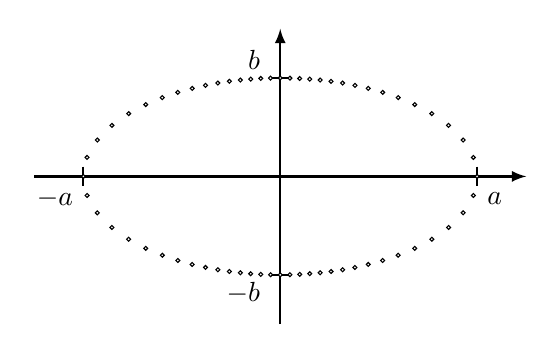
\begin{tikzpicture}
  \begin{scope}[scale = 2.5]
    \def\majradius{1}
    \def\minradius{0.5}
    \def\slingringsmonn{.25}
    \draw[-latex, thick] ({-\majradius - \slingringsmonn}, 0)--({\majradius + \slingringsmonn}, 0);
    \draw[-latex, thick] (0, {-\minradius - \slingringsmonn})--(0, {\minradius + \slingringsmonn});
    \draw[thick] ({-\majradius}, .05)--({-\majradius}, -.05) node[below = 1ex, left]{$-a$};
    \draw[thick] ({\majradius}, .05)--({\majradius}, -.05) node[below = 1ex, right]{$a$};
    \draw[thick] (.05, {\minradius})--(-.05, {\minradius}) node[above = 1.5ex, left]{$b$};
    \draw[thick] (.05, {-\minradius})--(-.05, {-\minradius}) node[below = 1.5ex, left]{$-b$};
    \def\numbernodes{64}
    \foreach \i in {0, ..., \numbernodes}
      \pgfmathsetmacro\teta{2 *\i * pi / \numbernodes}
      \def\radius{(\majradius*\minradius)/sqrt(\minradius^2 * (cos(\teta r))^2 + \majradius^2 * (sin(\teta r))^2)}
      \draw[fill = white] ({\radius*cos(\teta r)}, {\radius*sin(\teta r)}) circle (.01);
  \end{scope}
\end{tikzpicture}

  }
  \captionsetup{type = figure}
  \caption{Ellipse parametrized with the polar variable $\theta$, according to equation \eqref{eq:polar_ellipse}.}
  \label{fig:polar_ellipse}
\end{Figure}
We see that the points tend to accumulate at the top of the ellipse, which indeed makes sense.
As we change the polar angle by an equal amount counter-clockwise, the arc length drawn out between points will diminish towards $\sfrac{\pi}{2}$.
This is illustrated in figure \ref{fig:polar_arc_length_ellipse} below, where points on the ellipse for integer multiples of $\sfrac{\pi}{8}$ are plotted in the first quadrant.
\begin{Figure}
  \centering
  \scalebox{1}{%
    \begin{tikzpicture}
  \begin{scope}[scale = 5]
    \def\slingringsmonn{.2}
    \def\majorradius{1}
    \def\minorradius{.5}
    \draw[thick, -latex] ({-\slingringsmonn}, 0)--({\majorradius + \slingringsmonn}, 0);
    \draw[thick, -latex] (0, {-\slingringsmonn})--(0, {\minorradius + \slingringsmonn});
    \draw[thick] (\majorradius, .05)--(\majorradius, -.05) node[below]{$a$};
    \draw[thick] (.05, \minorradius)--(-.05, \minorradius) node[left]{$b$};
    \foreach \i in {0, ..., 4}
      \pgfmathsetmacro\teta{\i * pi / 8}
      \def\radius{(\majorradius*\minorradius)/sqrt(\minorradius^2 * (cos(\teta r))^2 + \majorradius^2 * (sin(\teta r))^2)}
      \draw[fill = white] ({\radius*cos(\teta r)}, {\radius*sin(\teta r)}) circle (.01);
  \end{scope}
\end{tikzpicture}

  }
  \captionsetup{type = figure}
  \caption{Demonstration that the arc length between points decreases counter-clockwise in the first quadrant as the polar angle $\theta$ approaches $\sfrac{\pi}{2}$.}
  \label{fig:polar_arc_length_ellipse}
\end{Figure}
This is not the case for the ellipse discretized according to equation \eqref{eq:parametric_ellipse}, using the eccentric variable $\eta$, as is seen in figure \ref{fig:eccentric_ellipse} below.
\begin{Figure}
  \centering
  \scalebox{1}{%
    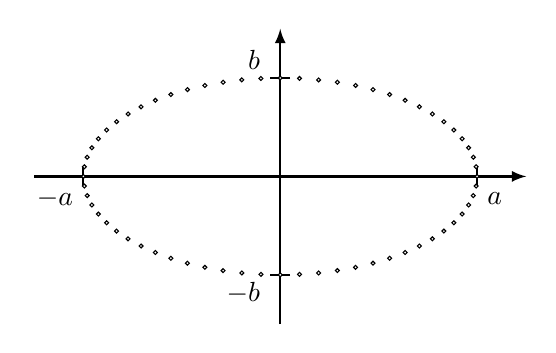
\begin{tikzpicture}
  \begin{scope}[scale = 2.5]
    \def\majradius{1}
    \def\minradius{.5}
    \def\slingringsmonn{.25}
    \draw[-latex, thick] ({-\majradius - \slingringsmonn}, 0)--({\majradius + \slingringsmonn}, 0);
    \draw[-latex, thick] (0, {-\minradius - \slingringsmonn})--(0, {\minradius + \slingringsmonn});
    \draw[thick] ({-\majradius}, .05)--({-\majradius}, -.05) node[below = 1ex, left]{$-a$};
    \draw[thick] ({\majradius}, .05)--({\majradius}, -.05) node[below = 1ex, right]{$a$};
    \draw[thick] (.05, {\minradius})--(-.05, {\minradius}) node[above = 1.5ex, left]{$b$};
    \draw[thick] (.05, {-\minradius})--(-.05, {-\minradius}) node[below = 1.5ex, left]{$-b$};
    \def\numbernodes{64}
    \foreach \i in {1, ..., \numbernodes}
      \draw[fill = white] ({\majradius*cos(2*\i*pi/\numbernodes r)}, {\minradius*sin(2*\i*pi/\numbernodes r)}) circle (.01);
  \end{scope}
\end{tikzpicture}

  }
  \captionsetup{type = figure}
  \caption{Ellipse parametrized with the eccentric variable $\eta$, according to equation \eqref{eq:parametric_ellipse}.}
  \label{fig:eccentric_ellipse}
\end{Figure}
\begin{Figure}
  \centering
  \scalebox{1}{%
    \begin{tikzpicture}
  \begin{scope}[scale = 5]
    \def\slingringsmonn{.2}
    \def\majorradius{1}
    \def\minorradius{.5}
    \draw[thick, -latex] ({-\slingringsmonn}, 0)--({\majorradius + \slingringsmonn}, 0);
    \draw[thick, -latex] (0, {-\slingringsmonn})--(0, {\minorradius + \slingringsmonn});
    \draw[thick] (\majorradius, .05)--(\majorradius, -.05) node[below]{$a$};
    \draw[thick] (.05, \minorradius)--(-.05, \minorradius) node[left]{$b$};
    \foreach \i in {0, ..., 4}
      \pgfmathsetmacro\teta{\i * pi / 8}
      \draw[fill = white] ({\majorradius*cos(\teta r)}, {\minorradius*sin(\teta r)}) circle (.01);
  \end{scope}
\end{tikzpicture}

  }
  \captionsetup{type = figure}
  \caption{Arc length increases counter-clockwise in the first quadrant as the eccentric variable $\eta$ approaches $\sfrac{\pi}{2}$.}
\end{Figure}
Of interest to investigate is how these distributions of nodes impact the convergence of the software---one thought is that performance of tendency for nodes to concentrate towards either of the semiaxes will positively impact the accuracy for the corresponding mode.
To be investigated is also whether a distribution such that arc lengths between nodes remain constant over the whole ellipse will perform better than either the eccentric or polar representation.

We wish to find a set of $N$ points on the ellipse such that the arc length between successive points is constant.
The arc length of a curve parametrized by $\bm{y}(x)$ is given by
\[
\ell(a;b) = \int_{a}^{b} \absl{\bm{y}^{\prime}(x)} \,\dee x, \qquad 0 \leq a \leq b,
\]
where $a$ and $b$ are the start and end points of the parametrization, and their ordering is convention for the sake of clarity.
Note that we may write $\ell(a;b) = \ell(0;b) - \ell(0;a) \equiv \ell(b) - \ell(a)$.
Finding then the arc length from $\eta = 0$ to some value, say $t$, using equation \eqref{eq:parametric_ellipse}, yields the integrand $\sqrt{a^2 \cos^2{\eta} + b^2 \sin^2{\eta}}$.
We may use the Pythagorean identity that $\cos^2{\eta} + \sin^2{\eta} = 1$, which yields
\[
\ell(\etatt) = a\int_{0}^{\etatt} \sqrt{1 - k^2 \sin^2{\eta}} \,\dee\eta, \qquad k^2 = 1 - \frac{b^2}{a^2},
\]
which is exactly the incomplete elliptic integral of the second kind, as written in equation \eqref{eq:incomplete_elliptic_integral_second}.
We now consider the perimeter of the ellipse.
Due to the symmetry of the ellipse---or the periodicity of the elliptic functions---it is evident that the perimeter is given by $\ell(2\pi) = 4\ellE(k)$.
We may then find the set of angles such that $N$ nodes of equal arc lengths are placed on the ellipse by the relation that
\[
\ellE(\etatt_n \vert k) = \frac{4n\ellE(k)}{a N}, \qquad n \in \{1, \dots, N\}.
\]
By an arithmetic-geometric mean algorithm, we may find the angles $\etatt$.
